%Template v.1.0: Taylor Arnold and Simon Gabay, december 2025
% CECI EST UN FICHIER DE MODÈLE LATEX POUR LES ARTICLES INCLUS DANS
% *Anthology of Computers and the Humanities*. AJOUTEZ L'OPTION
% 'final' LORS DE LA CRÉATION DE LA VERSION FINALE DE L'ARTICLE. 
% NE PAS modifier la classe du document
\documentclass[final, fra]{anthology-ch}     % pour la version finale
%\documentclass[fra, custom]{anthology-ch}      % pour la soumission

% CHARGER LES PACKAGES LaTeX
\usepackage{booktabs}
\usepackage{graphicx}
\usepackage{amsmath}
\usepackage{wrapfig}

% AJOUTEZ vos propres packages avec \usepackage{}

% TITRE DE LA SOUMISSION
% Remplacez ceci par le titre de votre soumission
\title{Traditions archivistiques et analyse computationnelle : modéliser les légendiers français à partir des données de Jonas}

% INFORMATIONS SUR LES AUTEURS ET LES AFFILIATIONS
% Pour chaque auteur, utilisez une nouvelle commande \author, avec
% les numéros entre crochets indiquant les affiliations correspondantes
% (section suivante) et l'ORCID-ID pour chaque auteur.  
\author[1]{Shannon Bruderer}[
  orcid=0000-0000-0000-0000,
  email=shannon.bruderer@msh-lse.fr
]

% Bien que nous encouragions l'ajout des ORCID-ID pour tous les auteurs, 
% vous pouvez inclure des auteurs qui n'en ont pas en laissant le champ vide.
\author[2]{Ariane Pinche}[
  orcid=0000-0002-7843-5050,
  email=ariane.pinche@cnrs.fr
]

% Il doit y avoir un appel à \affiliation pour chaque affiliation des auteurs.
% Plusieurs affiliations peuvent être attribuées à un auteur
% et une affiliation peut être attribuée à plusieurs auteurs. 
\affiliation{1}{Maison des Sciences sociales et des Humanités - Lyon St-Étienne, Lyon, France}
\affiliation{2}{CIHAM-UMR 5648, CNRS, Lyon, France}

% MOTS-CLÉS
% Fournissez un ou plusieurs mots-clés séparés par des virgules
% en utilisant les commandes suivantes
\keywords[fra]{humanités numériques, sciences humaines, base de données, philologie médiévale}
\keywords[eng]{digital humanities, humanities, database, medieval philology}

% MÉTADONNÉES DE LA PUBLICATION
% Ces champs seront remplis lors de la publication ; 
% ils peuvent être laissés par défaut lors de la soumission
\pubyear{2026}
\pubvolume{4}
\pagestart{166}
\pageend{174}
\paperorder{20}
\conferencename{Actes de la Conférence Humanistica}
\conferenceeditors{Serena Crespi, Simon Gabay, Martin Grandjean, Ariane Pinche, Marie Puren et Léa Saint-Raymond}
\doi{10.63744/87xcm3uNiTMz}
\customhead{}

\addbibresource{bibliography.bib}

%%%%%%%%%%%%%%%%%%%%%%%%%%%%%%%%%%%%%%%%%%%%%%%%%%%%%%%%%%%%%%%%%%%%%%%%%%%
% DÉBUT DU TEXTE
\begin{document}

\maketitle

\begin{abstract}
Nowadays, Digital Humanities are challenged by the growing prominence of computational and AI-based approaches, sometimes at the expense of data structuration. This article argues that rigorous data modelling remains a central epistemological component of Digital Humanities. Through the construction of a dynamic relational database dedicated to French medieval hagiographic manuscripts (legendiers), based on the metadata of the Jonas database (IRHT), we demonstrate how modelling choices in the database are intertwined with philological Issues. Focusing on the composition,  of legendiers, the article shows how standards-based modelling enables the analysis of textual variance, compilation logics, and manuscript relationships at multiple levels. By combining philological concepts with interoperable data structures, this work shows the importance of data modelling as an essential practice at the core of Digital Humanities research.
\end{abstract}

\section*{Introduction}

Une base de données peut être envisagée comme une représentation numérique d'un objet ou d'un concept. Par \og représentation \fg{}, nous entendons ici le travail de transposition qui consiste à rendre quelque chose présent sous la forme d'un substitut, en en restituant les composants, les traits et les caractéristiques, puis en explicitant la manière dont ceux-ci entrent en relation les uns avec les autres.

Il y a ainsi quelque chose de l'ordre de l'\og imitation \fg{} qui fonctionne comme une forme de traduction : la base de données transpose un objet inscrit dans le monde matériel vers un autre régime d'existence, celui d'une structure conceptuelle et formelle. Cela étant dit, et dans la mesure où le numérique lui-même repose sur des infrastructures physiques (serveurs, stockage, technologies), l'idée d'une supposée \og dématérialisation \fg{} peut être relativisée.

Toute la difficulté de ce travail réside dans la capacité à rendre compte d'une réalité complexe à travers une architecture qui impose ses propres traditions et modalités techniques. Toute modélisation suppose dès lors une série de choix : déterminer ce qui sera représenté, ce qui sera laissé en marge, et la manière dont les éléments retenus seront articulés entre eux et, par alignement, au-delà du système lui-même.

Les bases de données, en tant que structures organisées d'information, procèdent ainsi en deux temps. Premièrement, par décomposition : un objet est dissocié en un ensemble de propriétés distinctes. Deuxièmement, on en propose une nouvelle réécriture, où l'objet d'étude n'est pas simplement reproduit, mais décrit dans une forme qui n'est plus linéaire ou narrative, mais fragmentée, normalisée et interconnectée.

Au-delà de leur fonction de centralisation de l'information, les bases de données permettent de modéliser un objet à différentes échelles d'existence. Contrairement à l'idée selon laquelle le numérique induirait une forme d'absolutisme descriptif, souvent ressenti face aux choix de catégories qui semblent figer l'information dans sa qualification, la structuration des données introduit au contraire une finesse et une nuance accrues : un lieu, par exemple, peut être saisi simultanément à plusieurs niveaux, local comme global, et devient un label, une URI, des coordonnées ou encore un code multilingue et interopérable. Enfin, le caractère interrogeable de la base de données rend possible d'être simultanément précis et granulaire, tout en permettant une lecture généralisée des tendances lorsque l'on adopte une vue d'ensemble.

À travers la présentation des étapes de constitution d'une base de données relationnelle consacrée aux manuscrits hagiographiques français dits \og légendiers \fg{}, nous souhaitons montrer que ce travail  \og numérique \fg{} est étroitement lié à son objet d'étude, tant dans son existence matérielle que conceptuelle\footnote{Les données utilisées dans cette étude ainsi que les notebooks permettant leur traitement et leur analyse sont accessibles dans le dépôt suivant : \url{https://gitlab.huma-num.fr/sbruderer/legendier_manuscrit}.}. La base de données s'appuie sur les métadonnées de la base Jonas\footnote{Institut de Recherche et d'Histoire des Textes Section romane, \og JONAS - Section Romane - IRHT \fg{}, \url{https://jonas.irht.cnrs.fr}.}, qui ont été récupérées, restructurées et mises en relation de manière à pouvoir être analysées afin de mieux comprendre les légendiers français, leurs logiques de composition et leurs évolutions entre le \textsc{xiii}\ieme~ et le \textsc{xv}\ieme~siècle. Dans un premier temps, nous reviendrons sur les compilations hagiographiques et sur leurs enjeux philologiques ; nous présenterons ensuite les choix de modélisation opérés pour répondre au mieux aux questions de recherche ; enfin, nous proposerons une étude de cas afin d'illustrer la manière dont ces données peuvent être mobilisées.

\section{Les compilations hagiographiques françaises}\label{compilationHagiographiques}

Les Vies de saints ont connu une large diffusion au cours du Moyen Âge \cite{trigalet_compter_2001}, et ce, sous de multiples formes : textes unitaires, petits recueils thématiques ou d'auteur ou légendiers contenant des compilations de Vies de saints \cite{philippart_legendiers_1977}. Dans le cas des légendiers français, cette circulation s'accompagne d'une transformation de l'organisation de la compilation. Alors que les légendiers latins sont le plus souvent organisés selon le calendrier liturgique, les légendiers français du \textsc{xiii}\ieme~ siècle présentent majoritairement une organisation thématique (apôtres, martyrs, confesseurs et saintes femmes). Les premiers ensembles hagiographiques ont été classés en familles par P. Meyer \cite{meyer_legendes_1906}. Elles fonctionnent de manière cumulative : les légendiers de type A regroupent les Vies des apôtres, les légendiers  B associent apôtres et martyrs, les légendiers C apôtres,  martyrs, confesseurs et les saintes femmes, tandis que les autres familles sont constituées sur le modèle de C avec des ajouts de nouveaux textes. Au cours du \textsc{xiv}\ieme~s., les légendiers français tendent à revenir à une organisation liturgique. Ils proposent alors des versions abrégées des Vies de saints sur le modèle de la \textit{Legenda Aurea} de Jacques de Voragine, qui connaît un vif succès et fait l'objet de nombreuses traductions \cite{fleith_saintete_2001}.

Les légendiers contiennent des textes qui présentent des variations qu'il convient de prendre en compte afin de modéliser au plus près la mouvance propre aux textes médiévaux \cite{zumthor_intertextualite_1981}. En effet, ceux-ci sont constitués de textes qui narrent la vie d'un saint, comme la \textit{Vie de saint Lambert de Liège}. Cette trame narrative donne alors lieu à des mises en récit distinctes, produites par des auteurs différents qui, elles-mêmes, peuvent varier au cours des copies (variations graphiques, modernisation linguistique, erreurs, etc.). Ainsi, deux compilations peuvent partager une même trame narrative tout en intégrant des récits distincts, ce qui impose un niveau de granularité fin dans la modélisation.

Si la philologie traditionnelle s'est principalement appuyée sur l'unité textuelle afin d'analyser les relations entre les manuscrits, l'usage des méthodes numériques, et en particulier la modélisation au sein d'une base de données des traditions manuscrites, ouvre la possibilité d'aborder plus finement la transmission des textes au niveau des compilations et de prolonger les travaux fondateurs de Meyer, tout en offrant à la communauté scientifique un ensemble de données structuré, susceptible d'être réinvesti. Une telle démarche requiert une modélisation rigoureuse, ancrée à la fois dans les standards existants et dans les concepts philologiques, afin de constituer un outil scientifique pérenne et réutilisable.

\section{Du manuscrit à sa représentation numérique : standards et interopérabilité}\label{2RepresentationNumérique}

Dans le cadre de la modélisation de notre base de données, nous avons d'abord constitué un corpus initial de taille maîtrisable, tant du point de vue humain que computationnel, centré sur la présence de la \textit{Vie de Lambert de Liège} dans les compilations. En partant des identifiants Jonas des manuscrits pour aller vers leurs contenus et métadonnées, un travail de moissonnage des données du site Jonas a été réalisé. Celui-ci a mis en évidence l'importance des identifiants (ARK), des permaliens et d'un schéma de métadonnées stable, lesquels ont permis de récupérer un nombre considérable de données et de faire le pont entre plusieurs dépôts \footnote{Par exemple, le manuscrit Paris, Bibliothèque nationale de France, Manuscrits, fr. 00412 dispose d'une notice dans la base Jonas (\url{https://jonas.irht.cnrs.fr/consulter/manuscrit/detail_manuscrit.php?projet=45533}), d'un identifiant ARK dans la base ARCA (\url{https://arca.irht.cnrs.fr/ark:/63955/md182j62st0s}), d'un fac-similé numérique accessible sur Gallica (\url{https://gallica.bnf.fr/ark:/12148/btv1b84259980/f5.item}), d'une notice dans le catalogue Archives et Manuscrits de la BnF (\url{https://archivesetmanuscrits.bnf.fr/ark:/12148/cc50522d}), d'un manifeste IIIF (\url{https://iiif.biblissima.fr/collections/manifest/9024c5d42e7e08f849652ff9c8dac5bec28dec0c}), ainsi que d'une notice dans le portail Data Biblissima recensant les différents identifiants attribués au manuscrit (\url{https://data.biblissima.fr/w/Item:Q51134}). L'ensemble de ces dépôts témoigne de l'existence d'un environnement documentaire numérique vaste, dont le degré d'interconnexion reflète les efforts menés pour produire des données interopérables et conformes aux principes FAIR.}.

Après la collecte et le nettoyage des données, nous avons élaboré un premier modèle conceptuel. Celui-ci est centré sur les \og textes \fg{} au sein des manuscrits et mobilise des ontologies permettant un traitement normalisé des métadonnées associées aux documents. L'usage de vocabulaires normalisés assurent la désambiguïsation et préparent un requêtage apte à répondre à des questions en apparence simples portant sur les périodes de composition, les lieux, et les participants (auteur, commanditaire, copiste, etc.), qui sont essentielles dans l'étude des corpus \cite{hassner_computation_2013}. Conformément aux recommandations de FRBRoo, issues des pratiques bibliothéconomiques et du CIDOC-CRM, ancrées dans le champ de la conservation patrimoniale \cite{buard_modelisation_2015}, ainsi qu'à d'autres ontologies, le modèle s'organise autour de quatre grandes entités :

\begin{figure}[t!]
    \centering
    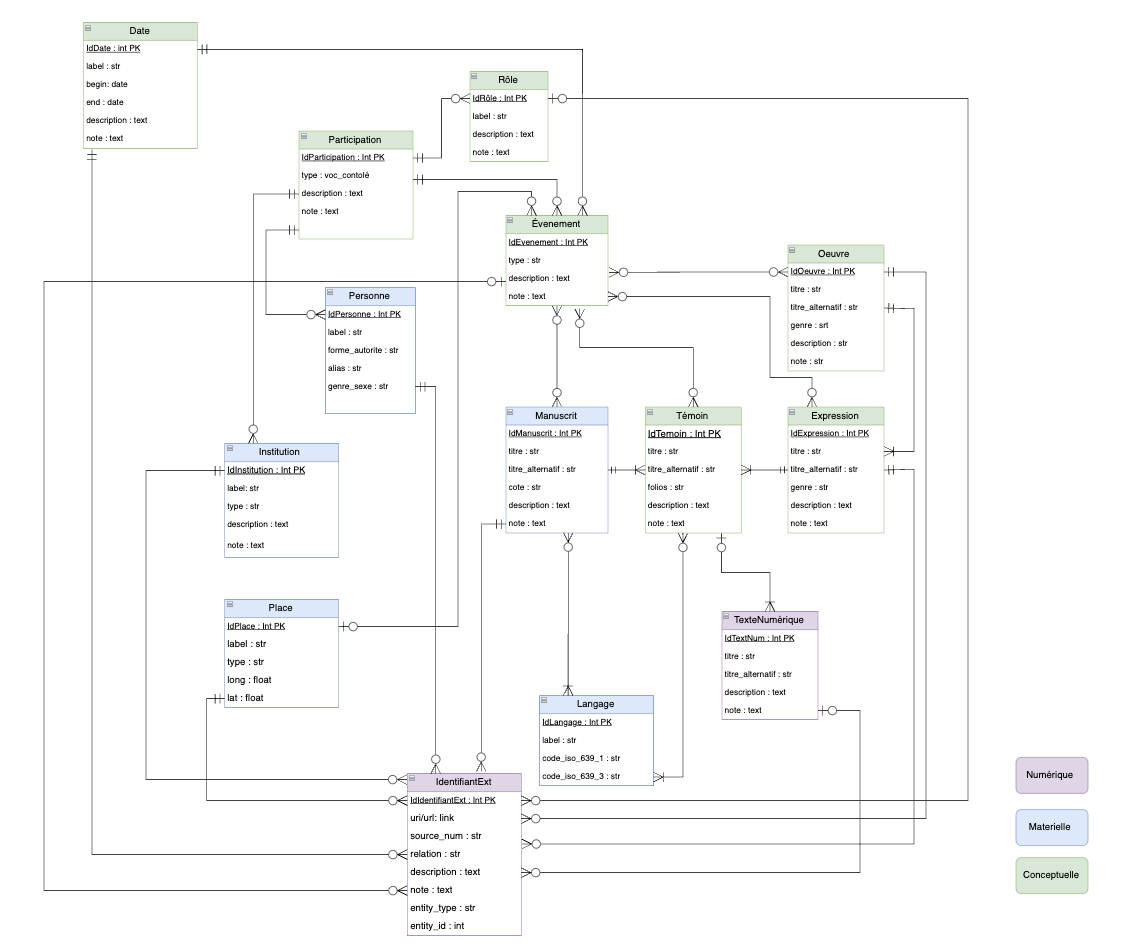
\includegraphics[width=\linewidth]{img/1_modeleBDD.png}
    \caption{Modèle logique de la base de données en notation \textit{Crow's Foot}.}
    \label{fig:modeleBDD}
\end{figure}

\vspace{0.3cm}
\begin{itemize}

\item l'\textit{\OE uvre} (F1 Work)\footnote{\url{https://cidoc-crm.org/f1-work}.}, définie comme une entité abstraite et immatérielle, correspondant ici à une trame narrative centrée sur une figure de saint.

\item l'\textit{Expression} (F2 Expression)\footnote{\url{https://cidoc-crm.org/f2-expression}.}, qui correspond à une réalisation intellectuelle de cette \oe uvre, c'est-à-dire une mise en récit particulière de la trame narrative. La relation entre l'\oe uvre et ses expressions peut être qualifiée par la propriété \textit{R19 created a realisation of (was realised through)}\footnote{\url{http://iflastandards.info/ns/fr/frbr/frbroo/R19}.}, qui permet de relier une \oe uvre abstraite aux différentes réalisations textuelles qui en dérivent.

\item le \textit{Témoin}, entendu comme l'attestation d'une expression donnée dans un support matériel précis (par exemple dans un manuscrit à une localisation donnée dans celui-ci). Cette entité permet de relier une expression abstraite à sa présence effective dans un document historique, tout en distinguant plusieurs attestations possibles d'une même expression. L'alignement ontologique du témoin pose toutefois question en raison de sa nature à la fois conceptuelle et matérielle. Afin de distinguer le contenu textuel du support qui le transmet, nous avons fait le choix d'aligner le témoin sur la classe \textit{E33 Linguistic Object}\footnote{\url{http://www.cidoc-crm.org/cidoc-crm/E33_Linguistic_Object}.} du CIDOC-CRM, qui permet de modéliser un contenu linguistique identifiable indépendamment de son support matériel. Dans ce cadre, le témoin correspond au texte attesté dans un manuscrit donné. Sa relation avec l'expression peut être qualifiée par la propriété \textit{R13 is realised in (realises)}\footnote{\url{http://iflastandards.info/ns/fr/frbr/frbroo/R13}.}, qui relie une expression à sa réalisation textuelle concrète.

\item la \textit{Manifestation Singleton} (F4 Manifestation Singleton)\footnote{\url{https://cidoc-crm.org/f4-manifestation-singleton}.}, entendue comme l'objet matériel unique dans lequel le texte est conservé, par exemple un manuscrit particulier. La relation entre le manuscrit et le témoin est exprimée par la propriété \textit{P128 carries (is carried by)}\footnote{\url{http://www.cidoc-crm.org/cidoc-crm/P128_carries}.}, le manuscrit étant ici compris comme le support matériel qui porte le contenu textuel attesté par le témoin.

\end{itemize}
\vspace{0.3cm}



\begin{figure}[t!]
    \centering
    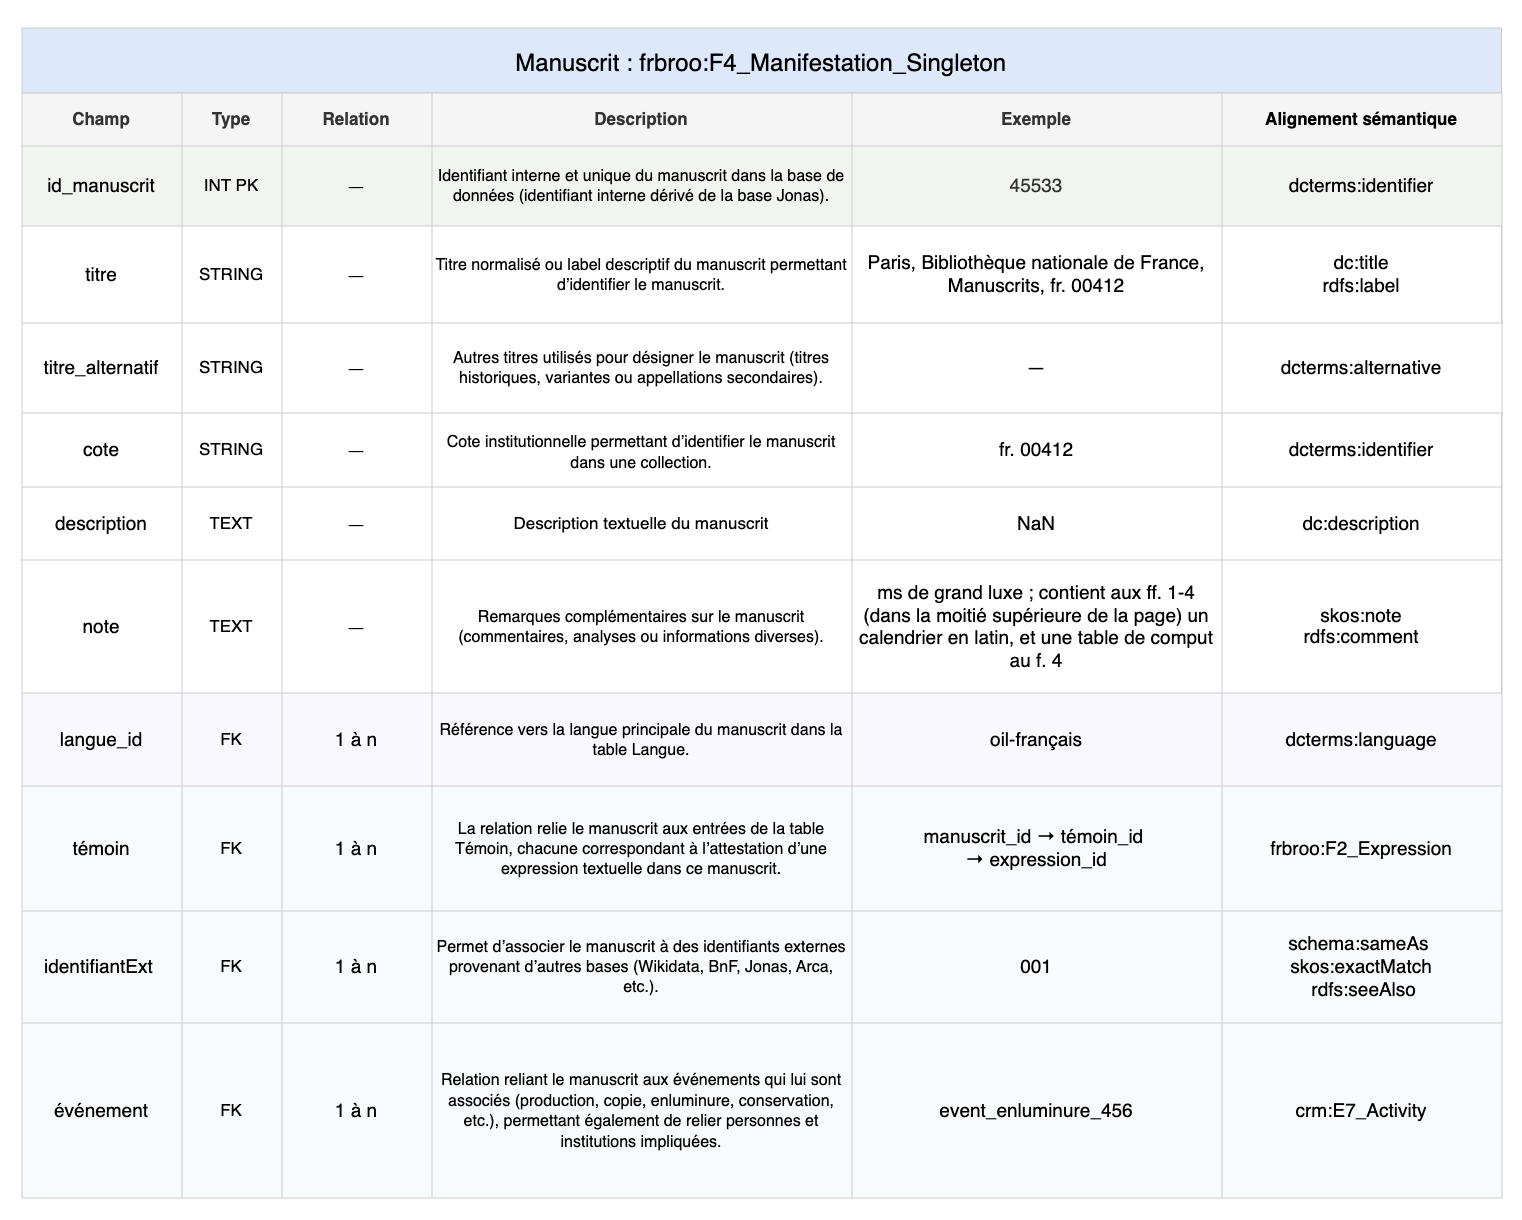
\includegraphics[width=\linewidth]{img/schema_02.png}
    \caption{Structure de la table \textit{Manuscrit} et alignement sémantique.}
    \label{fig:2rdf}
\end{figure}

Pour donner un exemple concret, la \textit{Vie de saint Lambert de Liège} constitue une \oe uvre comportant treize expressions recensées dans la base Jonas. Parmi celles-ci, on peut citer l'expression attribuée à Jean de Vignay\footnote{Anne-Françoise Leurquin et Marie-Laure Savoye, notice \textit{Vie de saint Lambert de Liège, Jean de Vignay}, base Jonas-IRHT/CNRS, \url{http://jonas.irht.cnrs.fr/oeuvre/3058}, consultation du 12/03/2026.} ou encore celle de Jeanne de Malone\footnote{Section romane, notice \textit{Vie de saint Lambert de Liège, Jeanne de Malone}, base Jonas-IRHT/CNRS, \url{http://jonas.irht.cnrs.fr/oeuvre/8764}, consultation du 12/03/2026.}. Cette dernière est attestée par un témoin conservé dans le manuscrit Leiden, Bibliotheek der Rijksuniversiteit, BPL 0046 A, aux folios 81vb--95vb. Dans la base de données, une table \textit{Texte Numérique}, alignée sur la classe \textit{Item}\footnote{\url{https://cidoc-crm.org/f5-item}.}, permet de distinguer la matérialisation textuelle unique attestée dans le manuscrit des différentes représentations numériques du texte. Les numérisations, les transcriptions ou encore les éditions encodées en TEI peuvent ainsi être référencées séparément et associées chacune à un identifiant unique, permettant de tracer les différentes formes de circulation et de transformation du texte.

\section{Analyse de réseau et logique de compilation des légendiers}

Nous avons réalisé de premières analyses quantitatives en exploitant les différentes tables de données et modélisé des familles de légendiers à l'aide de visualisations en graphe. Notre corpus se compose au total de 71 manuscrits. Parmi les manuscrits les plus fournis, on compte le British Library, Stowe MS 0050, le BnF, fr. 00416 et Bibliothèque de l'Arsenal, 3682 qui sont tous les trois des \textit{Légendes dorées} du 15\ieme\ siècle traduites par Jean de Vignay. Le plus petit légendier du corpus est celui de la Bibliothèque royale de Belgique, 10326 (Légendier de la famille B) (voir figure \ref{fig:3repartisionCroissant}).

\begin{figure}[htp]
    \centering
    \includegraphics[width=\linewidth]{img/schema_03.png}
    \caption{Répartition du nombre d'\oe uvres par manuscrit, classées par ordre croissant dans le corpus.}
    \label{fig:3repartisionCroissant}
\end{figure}

Dans notre corpus, 687 trames narratives distinctes ont été identifiées, correspondant au niveau de l'\textit{Œuvre}. Celles-ci donnent lieu à 2 653 expressions textuelles distinctes, chacune correspondant à une mise en récit particulière d'une même trame narrative. Enfin, ces expressions sont attestées par 11 038 occurrences textuelles dans les manuscrits du corpus.

\begin{wrapfigure}{r}{0.5\textwidth}
    \centering\vspace{-.4cm}
    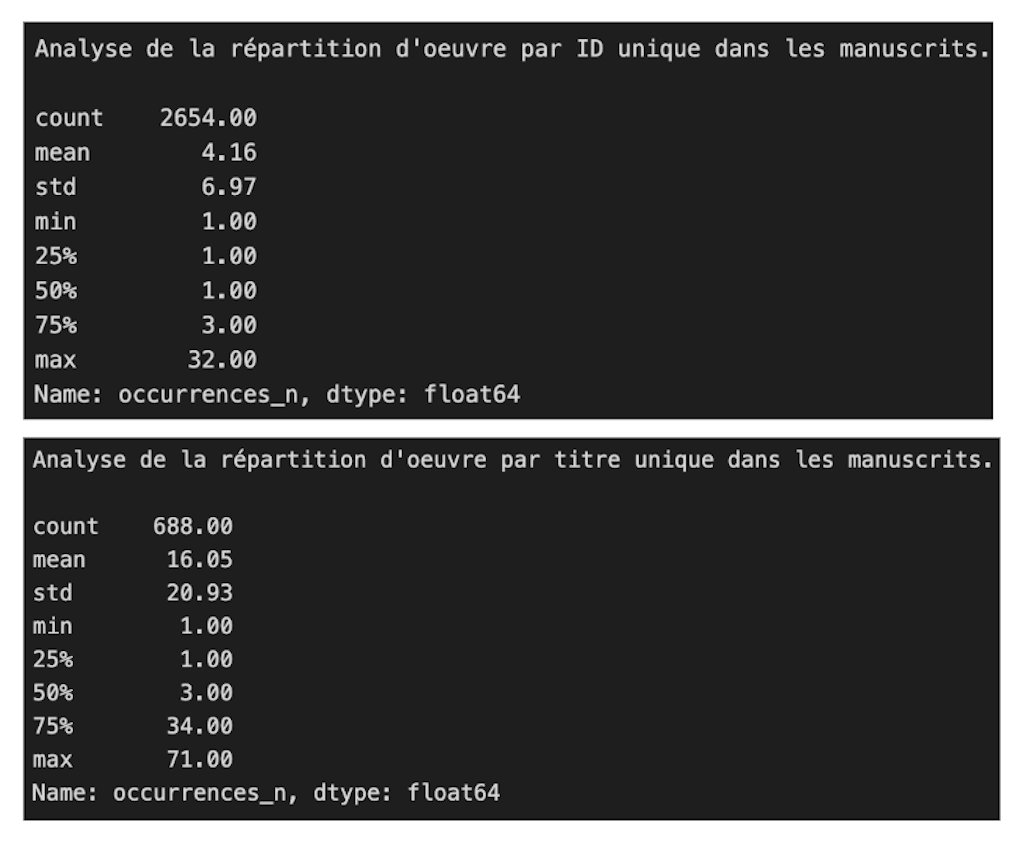
\includegraphics[width=\linewidth]{img/schema_04.png}
    \caption{Comparaison de la répartition du contenu des manuscrits selon un comptage par titre normalisé (trame narrative) ou par identifiant d’expression.}
    \label{fig:4repartition}
    \vspace{-.5cm}
\end{wrapfigure}

Comme nous l'avons mentionné précédemment (\ref{2RepresentationNumérique}), une même trame narrative peut se réaliser en plusieurs récits différents possédant chacun leur identifiant propre (voir section \ref{compilationHagiographiques}). En effet, la \textit{Vie de saint Lambert de Liège} connaît treize mises en récit distinctes, parfois sensiblement différentes \cite{clerice_wauchier_2025}. La version ancienne porte l'identifiant 1958 dans la base Jonas, tandis qu'une autre version, correspondant à la traduction par Jean de Vignay de la version latine de la \textit{Legenda aurea}, porte l'identifiant 3058.

Si la première question adressée aux données est relativement simple -- à savoir comment les \oe uvres se répartissent à travers les manuscrits --, sa réponse met en évidence un écart important dans les résultats selon que l'on considère l'identifiant attribué aux récits (c'est-à-dire aux expressions) ou que l'on regroupe les données selon leur titre comme référence, analysant ainsi la trame narrative, soit l'\oe uvre\footnote{La question se complique encore si plusieurs saints portent le même nom, comme c'est le cas pour saint Grégoire, le pape, l'auteur et le bon pécheur.}. En effet, en prenant appui sur le titre, un total de 687 \oe uvres se répartissent entre les manuscrits avec en moyenne d'apparition dans le corpus de 16\%. Dans cette perspective le troisième quartile est à 34, ce qui signifie que 25\% des \oe uvres sont attestées plus de 34 fois (voir figure \ref{fig:4repartition}). Ici, la \textit{Vie de saint Matthieu} et la \textit{Vie de saint Lambert de Liège} sont les plus répétées\footnote{Ce qui est relativement normale car l\textit{a Vie de saint Lambert de Liège} a servi à la constitution du corpus.}. 

Si nous examinons les expressions à partir de leur identifiant, les récits de la \textit{Vie de saint Clément} ou la \textit{Commémoration des défunts} dominent le corpus (chacune présente dans trente-deux manuscrits), leur trame narrative s'étant réalisée dans un nombre relativement limité de mises en récit différentes.



Grâce au jeu de données, une première visualisation des logiques de compilation des légendiers a été réalisée. Nous avons élaboré un graphe traduisant les relations qu'entretiennent les manuscrits, en fonction des contenus qu'ils partagent. Plusieurs étapes de préparation ont été indispensables, dont l'ajout d'une colonne titre\_id. Elle nous a permis d'attribuer à l'ensemble des \oe uvres un identifiant fondé sur le titre, afin de rendre compte des logiques de compilation, non pas uniquement des versions textuelles, mais aussi au niveau des trames narratives (F1 Work). En effet, les \oe uvres (trames narratives) correspondant à un même titre ont ainsi été regroupées sous un identifiant commun, afin de permettre un second niveau d'analyse de compilation des légendiers\footnote{Si jamais un copiste conservait la même compilation, mais pour une raison ou une autre décide d'insérer une autre version d'un texte.}. Nous avons ainsi construit un graphe bipartite dans lequel les n\oe uds sont répartis en deux ensembles distincts : les manuscrits d'un côté et les trames narratives de l'autre. À ce stade, les relations manuscrit-manuscrit sont indirectes et transitent par les n\oe uds représentant les trames narratives qui servent de n\oe uds-ponts. La proximité entre deux manuscrits est ensuite calculée à partir du nombre de trames narratives partagées $(weight(M1,M2)=\mid O(M1)\cap O(M2)\mid)$, ce qui définit le poids du lien dans le graphe projeté et permet l'identification de clusters de manuscrits. 

\begin{wrapfigure}{r}{0.5\textwidth}
    \centering\vspace{-.3cm}
    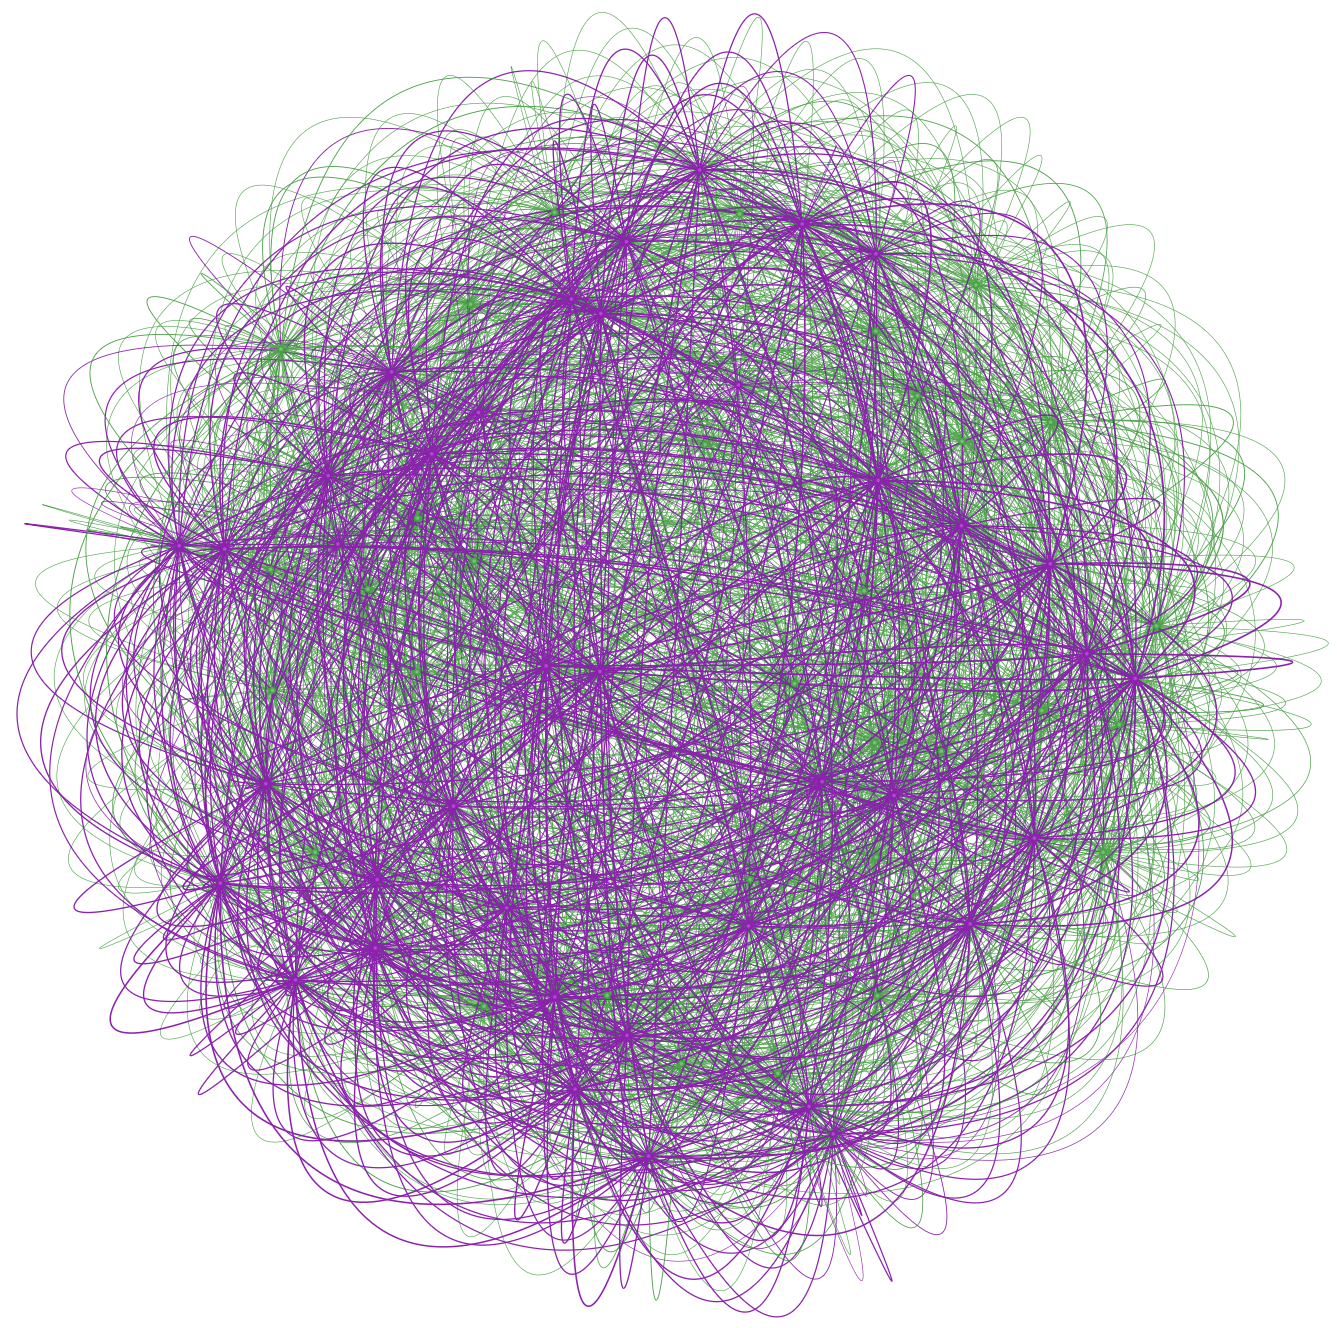
\includegraphics[width=\linewidth]{img/Schema_05.png}
    \caption{Graphe des relations entre manuscrits fondé sur le partage des trames narratives.}
    \label{fig:5graph}
    \vspace{-.3cm}
\end{wrapfigure}

Le graphe bipartite initial comporte 758 n\oe uds (trames narratives et manuscrits), ce qui correspond à l'ensemble des 687 trames et des 71 manuscrits du corpus. Une fois le graphe projeté, les résultats montrent une forte standardisation des légendiers : le graphe manuscrit–manuscrit compte 71 n\oe uds et 2 485 arêtes, indiquant que la quasi-totalité des manuscrits partage au moins une trame avec les autres. Les statistiques montrent également que la moitié des paires partagent plus ou moins 75 titres entre eux, le maximum est de 226, le minimum de 6. Certains manuscrits comme Thüringer Universitäts -- und Landesbibliothek, Ms. El. f. 86 et BnF, fr. 00416 possèdent des compilations presque identiques avec 226 \oe uvres partagées. L'analyse permet d'identifier deux clusters, respectivement composés de 39 et 32 manuscrits, ce qui souligne l'existence d'une logique de compilation largement partagée entre les manuscrits (voir figure 
\ref{fig:5graph}). En raison de la forte densité du réseau, causée par la présence de trames narratives communes largement diffusées, les deux principales familles ne sont distinguables que par leur couleur. 

\begin{wrapfigure}{r}{0.5\textwidth}
    \centering\vspace{-.3cm}
    \includegraphics[width=\linewidth]{img/Schema_06.png}
    \caption{Graphe des relations entre manuscrits fondée sur le partage des expressions.}
    \label{fig:6graph}
    \vspace{-.3cm}
\end{wrapfigure}

En comparaison, le graphe basé sur les différentes expressions d'une même trame narrative propose une autre visualisation des relations entre les manuscrits. Comportant 2 724 n\oe uds, il se compose de cinq clusters, regroupant respectivement 31, 28, 9, 2 et 1 manuscrits (voir figure \ref{fig:6graph}). Cette visualisation souligne combien le niveau d'analyse retenu influe sur la représentation des relations entre les manuscrits. Les deux niveaux coexistent en effet simultanément dans les sources, ce qui montre l'intérêt d'une modélisation capable de rendre compte de ces différentes échelles d'existence du texte.

L'une des perspectives de travail consisterait à filtrer les trames les plus fréquentes afin d'atténuer le poids du standard imposé par ces textes communs et de faire émerger des liens plus spécifiques. Cette approche repose sur l'hypothèse que, dans des pratiques de compilation fortement standardisées, ce sont les entrées rares qui témoignent d'une proximité plus significative entre les manuscrits\footnote{Nous avons mené la même expérience à partir des différents récits des Vies (expressions), en initiant les regroupements à un seuil de dix Vies partagées. Cette approche a permis de dégager trois clusters. Après vérification à partir de la \textit{Vie de saint Lambert}, chaque cluster semble associé à des mises en récit spécifiques, montrant que la transmission de ces textes ne s'opère pas principalement à l'échelle du texte isolé, mais bien à celle de la compilation.}.

%// (voire le csv “lien_manuscrit_vf.csv” qui récapitule tout les poids entre 2 manuscrits)
%Construire le graphe manuscrit↔manuscrit (projection), poids = nb d'\oe uvres partagées
%/// Graphe viz_manuscrits_projection.html
%//\newpage
\section*{Conclusion}

Si plusieurs pistes quant à l'analyse des logiques de compilation ont déjà été évoquées, ce travail appelle également des analyses textuelles plus fines. Notamment avec la mise en ligne récente de CoMMA, qui donne accès à la transcription de plus de 30 000 manuscrits \cite{clerice_comma_2025}, il serait possible d'élargir l'étude et de dépasser des analyses uniquement basées sur les métadonnées pour s'orienter vers des méthodes computationnelles appliquées au texte lui-même : analyse du nombre de tokens, mesure du \textit{token overlap}, ou encore calcul de similarités cosinus. Ces approches permettraient de proposer des analyses à plusieurs niveaux, de la trame narrative aux témoins manuscrits.

Plus largement, ce travail met en évidence la zone d'intersection dans laquelle se situent les humanités numériques. La juxtaposition des termes \og humanités \fg{} et \og numériques \fg{} engage, depuis l'émergence de la discipline, de longues discussions sur la compatibilité de ces deux \og mondes \fg{}. Cependant, nous avançons que, dans un environnement archivistique qui tend vers l'interconnexion de ses données, les frontières deviennent plus floues. Pour la constitution de notre base de données, il a en effet été indispensable de croiser trois champs de réflexion majeurs : la matérialité de l'objet manuscrit, ses spécificités conceptuelles autour de la notion de \og texte \fg{}, et son contexte numérique. Chacune de ces dimensions s'est trouvée intégrée au modèle conceptuel, non comme un simple ajout, mais comme un élément structurant.

Il convient toutefois de souligner que ce processus est loin de suivre un déroulement linéaire allant de la collecte des données au traitement, puis à l'analyse. La pratique a montré que le travail sur les données repose au contraire sur de constants allers-retours entre ces différentes phases. Bien souvent, ce sont les premiers résultats quantitatifs ou les visualisations issues des méthodes computationnelles qui révèlent des incohérences, des défauts de normalisation ou des indexations inadéquates. La réalité professionnelle des ingénieur·es en humanités numériques, amené·es à intervenir à différents niveaux de complexité, montre que la maîtrise des traditions archivistiques et une connaissance du document restent des conditions essentielles à la production d’analyses pertinentes.

Enfin, ce travail rappelle que les opérations dites \og manuelles \fg{} ou de base sur les données, comme le nettoyage, l'harmonisation ou la documentation, ne constituent pas une étape secondaire, mais forment le socle même à partir duquel des analyses solides, d'un point de vue computationnel comme disciplinaire, peuvent émerger.


% Imprime la bibliographie à la fin. Gardez cette ligne après le texte
% principal de votre article et avant une annexe.
\printbibliography

% Vous pouvez inclure une annexe en utilisant la commande suivante
\appendix



\end{document}